



\begin{frame}{\citetitle{MarcoNuno_CongArbEsp_2019_09_01} \footnotemark (1)}
\begin{columns}
\begin{column}{0.6\textwidth}
Los componentes de la báscula inteligente son:
	\begin{itemize}
\item Báscula digital
\item Sensor ultrasónico
\item Cámara
\item Pantalla touch
\item Operada por comandos por voz
\item Controlada por una computadora embebida con conexión a internet (Raspberry-Pi)
	\end{itemize}
\end{column}
\begin{column}{0.4\textwidth}
\begin{center}
     %%%%% this is a minipage, so \textwidth is already adjusted to the size of the column
     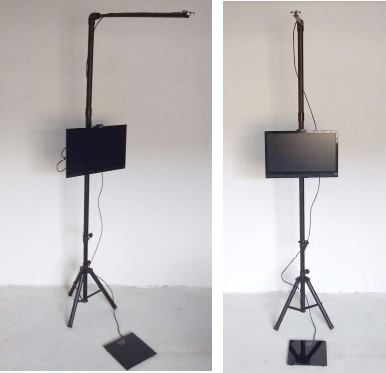
\includegraphics[width=0.99\textwidth]{Figs/Bascula1}
     \end{center}
\end{column}

\end{columns}
\footnotetext[1]{\fullcite{MarcoNuno_CongArbEsp_2019_09_01}}
\setcounter{footnote}{0}
\end{frame}

\begin{frame}{\citetitle{MarcoNuno_CongArbEsp_2019_09_01} (2)}
\begin{columns}
\begin{column}{0.35\textwidth}
La interfaz mostrada:
	\begin{itemize}
\item Estima los parámetros obtenidos
\item Estima el Indice de Masa Corporal (IMC)
\item Propone un régimen alimenticio (se recomienda consultar a un especialista)
	\end{itemize}
\end{column}
\begin{column}{0.65\textwidth}
\begin{center}
     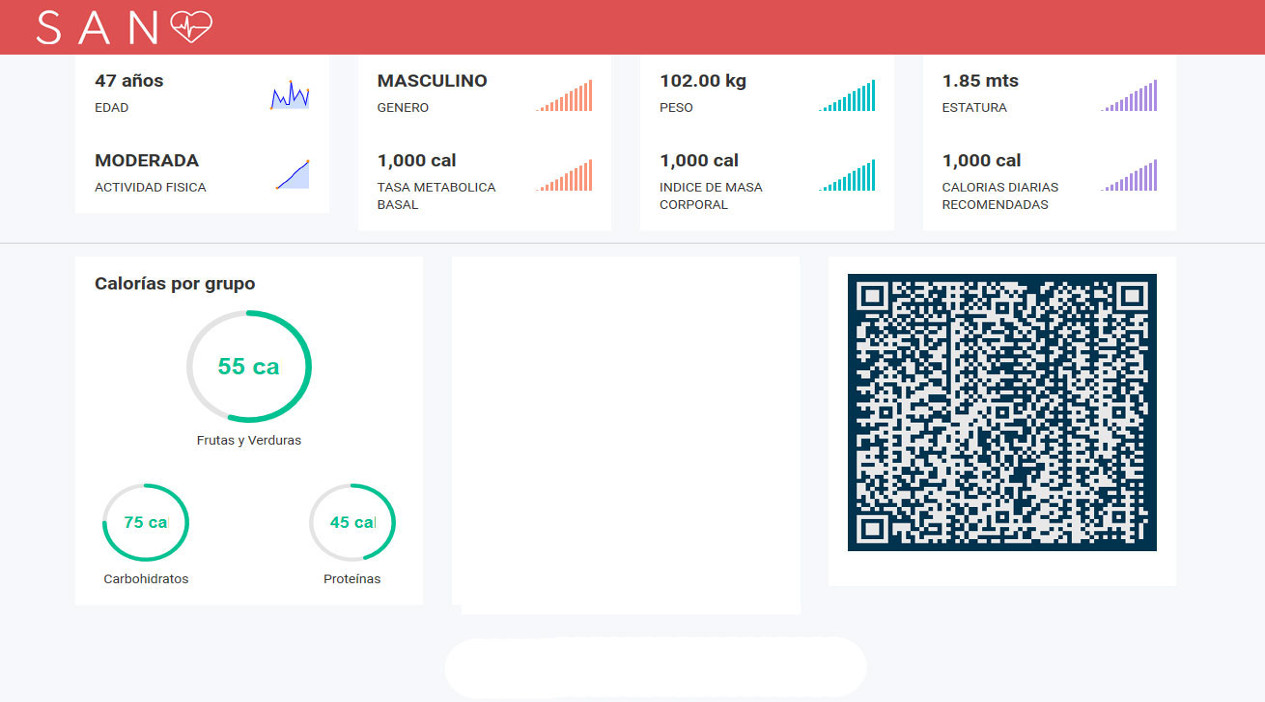
\includegraphics[width=0.99\textwidth]{Figs/Bascula2}
     \end{center}
\end{column}

\end{columns}
\end{frame}



